\documentclass[]{article}
\usepackage{caption,subcaption,graphicx,float,url,amsmath,amssymb}
\usepackage[hidelinks]{hyperref}
\usepackage[toc,acronym,nonumberlist]{glossaries}
\setacronymstyle{long-short}
\usepackage{glossaries-extra}
\graphicspath{{figs/}} 
\renewcommand{\thesection}{3.\arabic{section}}

%opening
\title{
	Notes from Origins of Life\\
	Week 3: Chemical Commonalities
}
\author{Simon Crase}

\makeglossaries

\loadglsentries{glossary}

\renewcommand{\glstextformat}[1]{\textbf{\em #1}}

\begin{document}

\maketitle

\begin{abstract}
 	These are my notes from Week 3 of the \gls{gls:SFI} Origins of Life Course\cite{sfi2019}. The course aims to push the field of Origins of Life research forward by bringing new and synthetic thinking to the question of how life emerged from an abiotic world.\\
  	The content and images contained herein are the intellectual property of the Santa Fe Institute, with the exception of any errors in transcription, which are my own.
  	These notes are distributed in the hope that they will be useful,
  	but without any warranty, and without even the implied warranty of
  	merchantability or fitness for a particular purpose. All feedback is welcome,
  	but I don't necessarily undertake to do anything with it.
\end{abstract}

\setcounter{tocdepth}{2}
\tableofcontents

\listoffigures

\section{Introduction}

This week is a more detailed look at biochemistry: biological information encoded in chemistry; the chemical processes that drive organization; and how life extracts energy from its environment.

\section{DNA as Information}
Lecturer: Michael Lachmann, \gls{gls:SFI}

\subsection{DNA Modification}

\begin{figure}[H]
	\caption{The 4 Nucleotides in DNA}\label{fig:Nucleotides} 
	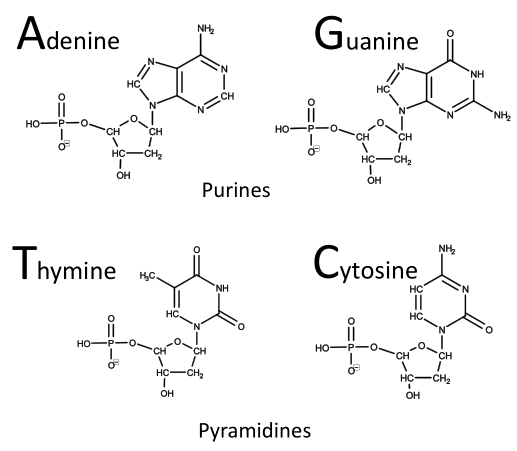
\includegraphics[width=0.9\textwidth]{Nucleotides}
\end{figure}

\begin{figure}[H]
	\caption{A closer look at one Nucleotide, Adenine}\label{fig:NucleotideAdenine} 
	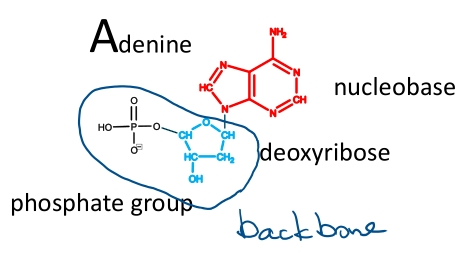
\includegraphics[width=0.9\textwidth]{NucleotideAdenine}
\end{figure}

Figure \ref{fig:NucleotideDNARNA} shows the only chemical difference between DNA and RNA: the extra OH group in RNA, which makes the molecule more active. DNA is more stable.
\begin{figure}[H]
	\caption{The only chemical difference between DNA and RNA }\label{fig:NucleotideDNARNA} 
	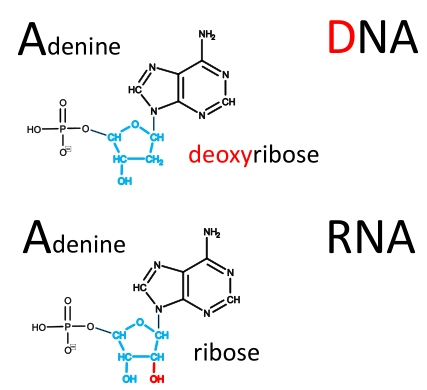
\includegraphics[width=0.9\textwidth]{NucleotideDNARNA}
\end{figure}

RNA uses Uracil instead of Thymine--Figure \ref{fig:NucleotideDNARNAThymineUracil}. Note that Thymine is Uracil with an extra methyl group, hence the alternative name $5-methyluracil$. The $5$ comes from the numbering of carbon atoms--see \ref{fig:NucleotidesCounting}
	
\begin{figure}[H]
	\caption{RNA uses Uracil instead of Thymine.} \label{fig:NucleotideDNARNAThymineUracil} 
	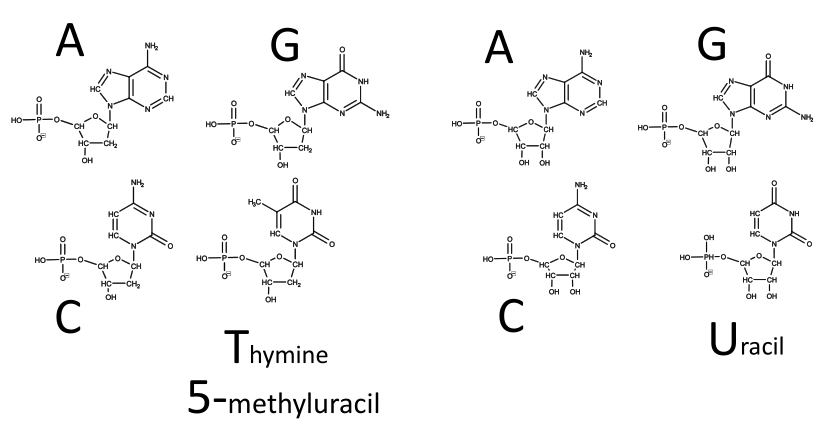
\includegraphics[width=0.9\textwidth]{NucleotideDNARNAThymineUracil}
\end{figure}

\begin{figure}[H]
	\caption{Numbering of carbon atoms in purines and pyrimidines. }\label{fig:NucleotidesCounting} 
	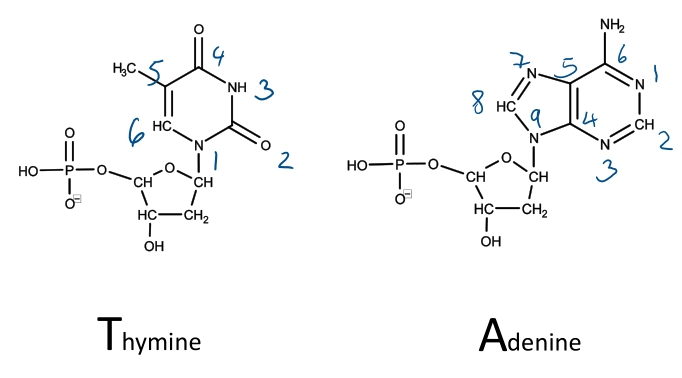
\includegraphics[width=0.9\textwidth]{NucleotidesCounting}
\end{figure}

\begin{figure}[H]
	\caption{A selection of 12 modified bases}\label{fig:ModifiedBases} 
	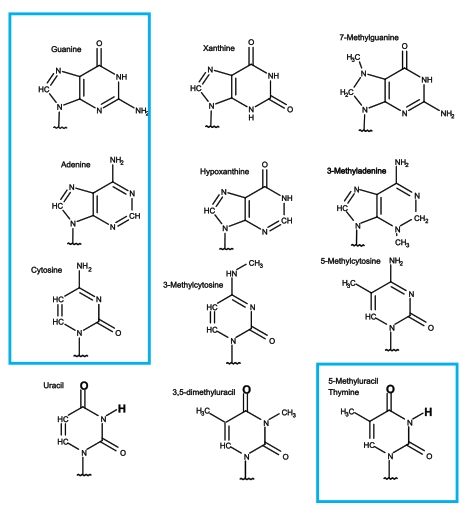
\includegraphics[width=0.9\textwidth]{ModifiedBases}
\end{figure}

\gls{gls:deamination}

Fugre \ref{fig:ModifiedDNA_Nucleobases} shows the 44 Modified DNA nucleobases that have actually been observed.\cite{sood2019dnamod},\cite{sood2019dnamod_website}

\begin{figure}[H]
	\caption{Modified DNA nucleobases } \label{fig:ModifiedDNA_Nucleobases} 
	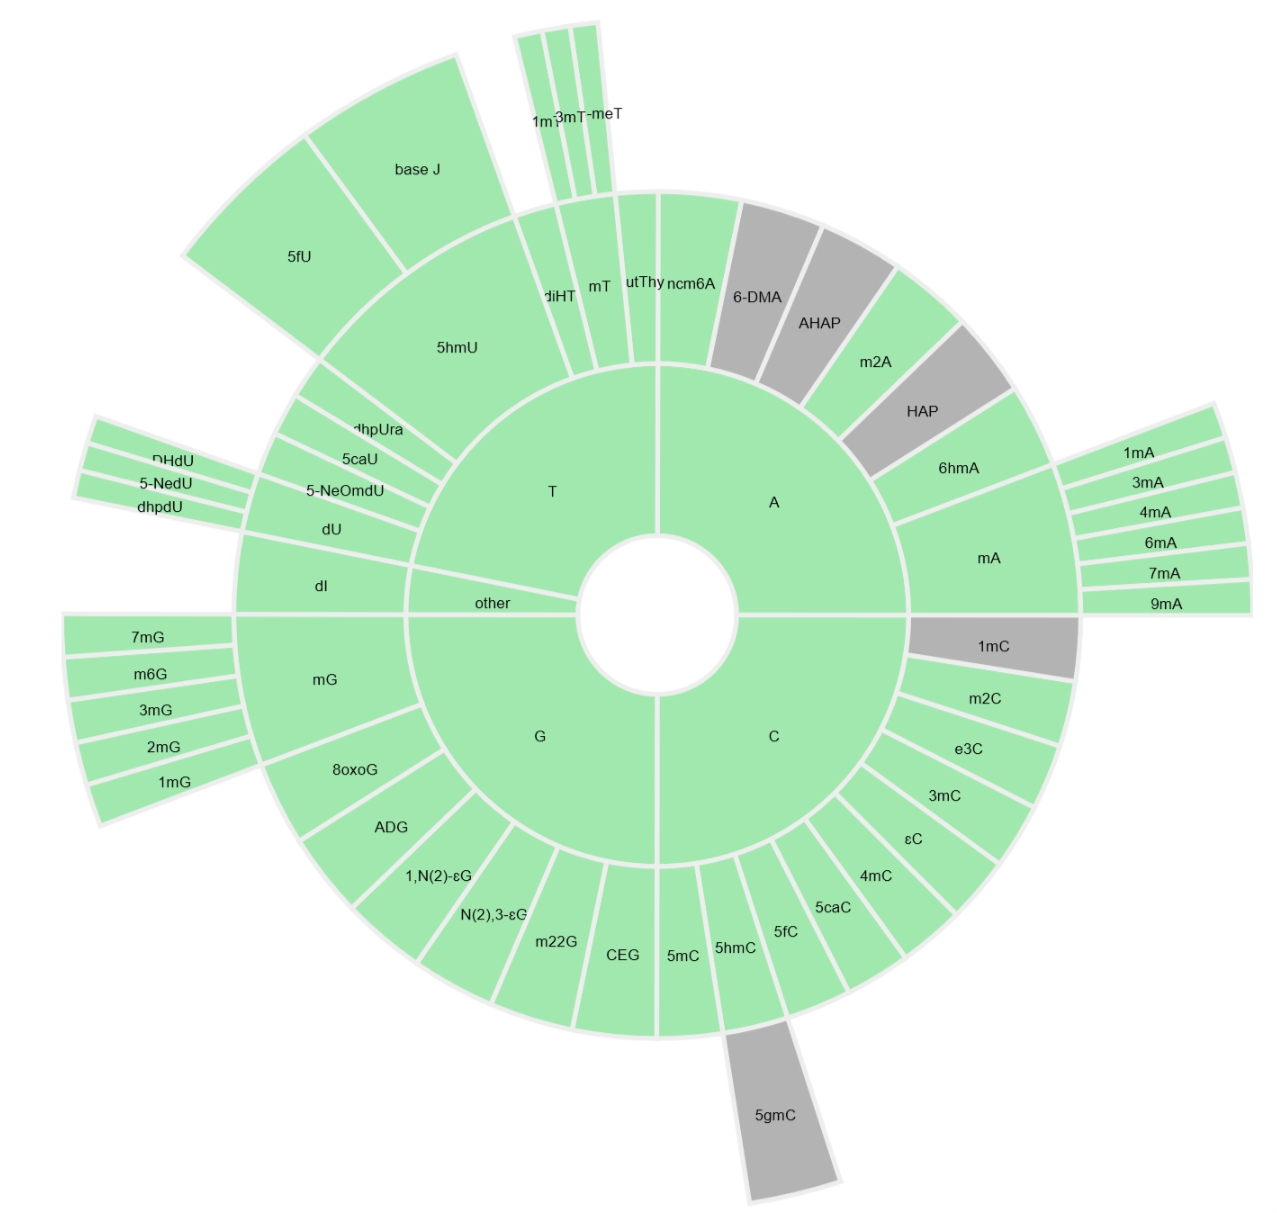
\includegraphics[width=0.9\textwidth]{ModifiedDNA_Nucleobases}
\end{figure}

The are a couple of bacteriophages, PBS1 and PBS2, that contain Uracil instead of thymine in their DNA\cite{hemphill1975bacteriophages}. Either the thymine has been replaced, or these phages are more primitive, and never used thymine.

When people talk about methylation of DNA, they usually mean $5-methylcytosine$, Figure \ref{fig:5methylcytosine}, even though there are many other ways to do it
\begin{figure}[H]
	\caption{$5-methylcytosine$ } \label{fig:5methylcytosine} 
	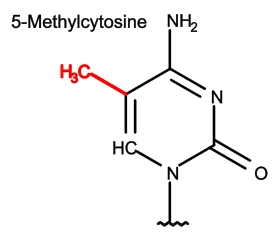
\includegraphics[width=0.9\textwidth]{5-methylcytosine}
\end{figure}

Methylation tends to occur when C is followed by G. The methylated versions are replicated us unmethylated C, but there is an enzyme, \gls{gls:DNAmethyltransferase}, which performs methylation, as shown in Figure \ref{fig:5-methylcytosine-in-action}. This can carry epigenetic changes across cell divisions, and sometimes across generations. This is important as it means that a lever cell can "remember" that is comes from a liver cell.
\begin{figure}[H]
	\caption{Methylation tends to occur when C is followed by G } \label{fig:5-methylcytosine-in-action} 
	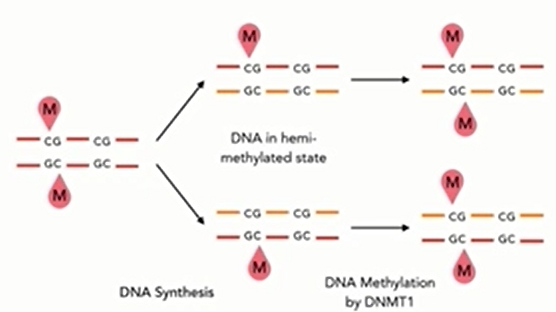
\includegraphics[width=0.9\textwidth]{5-methylcytosine-in-action}
\end{figure}

6-Methyladenine is also important--Figure \ref{fig:6-Methyladenine}-- in bacteria, where it carries information regarding the old strand versus the new. The methylation isn't very fast, so it can distinguish old from new. Section \ref{section:DNAasInfo2} shows how this is useful for repair.

\begin{figure}[H]
	\caption{6-Methyladenine is also important (palindromic sequence)} \label{fig:6-Methyladenine} 
	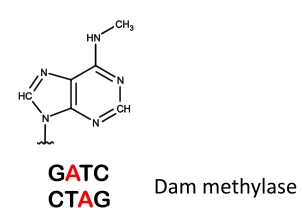
\includegraphics[width=0.9\textwidth]{6-Methyladenine}
\end{figure}

The values in Figure \ref{fig:ModifiedRNAdatabase} have been taken from the Modified RNA database \cite{agriss2019RNA}.

\begin{figure}[H]
	\caption{Modified RNA database} \label{fig:ModifiedRNAdatabase} 
	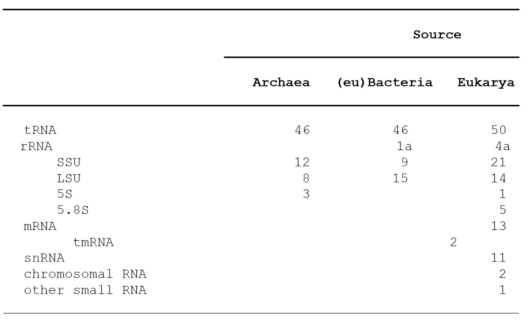
\includegraphics[width=0.9\textwidth]{ModifiedRNAdatabase}
\end{figure}

\textbf{Summary}

\begin{itemize}
	\item There are 44 known DNA modifications
	\item There are 112 known RNA modifications
	\item Many DNA modifications survive replication
	\item Some are replicated themselves
	\item Some modifications are functional:\begin{itemize}
		\item 5-methylcytosine (5mC)
		\item N6-methadenine (6mA)
		\item 5-hydroxymethylcytosine (5hmC)
		\item Some functional in RNA
		\item It is likely there are more, since this is a fairly new field.
	\end{itemize}
	\item How are they generated?
\begin{itemize}
	\item Enzyme activity
	\item Damage
	\item Misincorporation
\end{itemize}
\end{itemize}

Where did the modifications come from? They could be fairly new, and we use them in various ways; or maybe they tell us something about the origin of DNA. Maybe there are many enzymes left over from before we had sophisticated machinery for DNA replication.

\subsection{DNA base pairing}\label{section:DNAasInfo2}

What generates and maintains the pairing rules?  How does DNA keep Error rate down to  $10^{-10}$ errors per (replication*base pair)?

Different pairing proceed at different rates--Figures \ref{fig:RightWrong} and \ref{fig:BindingDifference}, but this won't explain error rate of $10^{-10}$. At best it gives a factor of 60.
\begin{figure}[H]
	\caption{Different pairing proceed at different rates} \label{fig:RightWrong} 
	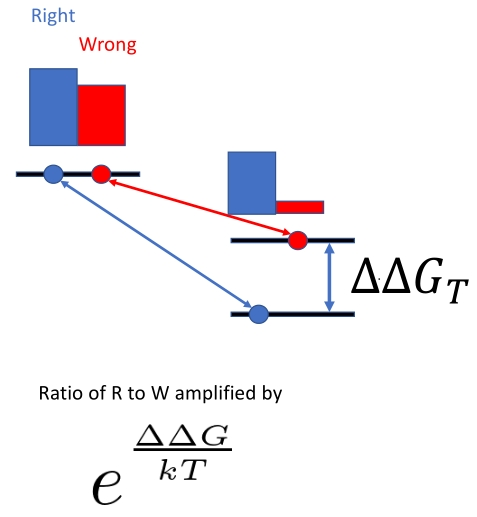
\includegraphics[width=0.9\textwidth]{RightWrong}
\end{figure}

\begin{figure}[H]
	\caption{Difference in Binding Energies for different pairings} \label{fig:BindingDifference} 
	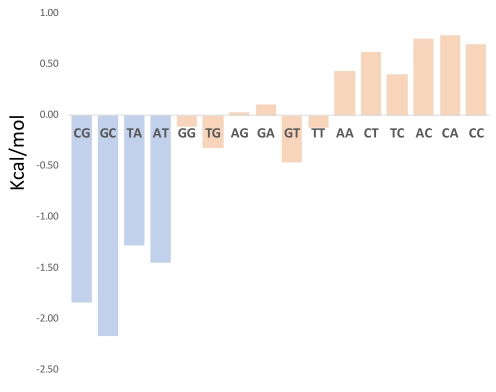
\includegraphics[width=0.9\textwidth]{BindingDifference}
\end{figure}
 Kinetic proofreading?
 
 
\textbf{Bases encountered by DNA polymerase}
	
\begin{itemize}
	\item Watson Crick pairs (CATG)
\begin{itemize}
	\item  Only ~50 fold enrichment from pairing
	\item  Right base at 3-fold disadvantage
	\item  4 shapes valid
\end{itemize}
	\item  “Valid” W-C extra bases (C*,6mA)
	\begin{itemize}
		\item Additional shapes valid
	\end{itemize}
	\item NTP from RNA
	\begin{itemize}
		\item Frequent
		\item Shape recognition
	\end{itemize}
	\item “Nonstandard” bases
	\begin{itemize}
		\item Rare, probably shape recognition
	\end{itemize}
\end{itemize}


Summary – it isn’t in the bases
\begin{itemize}
	\item Many bases exist in DNA/RNA
	\begin{itemize}
		\item Damage, modification, insertion
	\end{itemize}
	\item dNTP concentration is controlled
	\item DNA polymerase controls	pairing
	\item Large number of specific/general repair enzymes
\end{itemize}
\cite{kunkel2004dna}

\section{Water as a Driving Force for Organization}

Sarah Maurer

\begin{figure}[H]
	\caption{Chemical Energetics} \label{fig:ChemicalEnergetics} 
	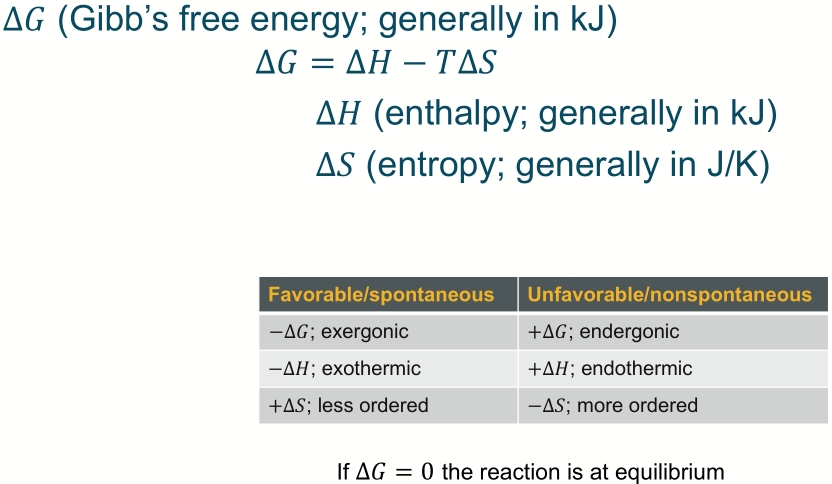
\includegraphics[width=0.9\textwidth]{ChemicalEnergetics}
\end{figure}

 Relevance to origins of life?
\begin{itemize}
	\item Are proteins necessary in first life?
	\item Membranes?
	\item Is water necessary for life?
\end{itemize}

\cite{ball2017water}

\section{Kinetic vs. Thermodynamics – Assembly Constraints}

Lecturer: Chris Butch

\begin{itemize}
	\item \gls{gls:kinetics}  \glsdesc{gls:kinetics}
	\item \gls{gls:thermodynamics} \glsdesc{gls:thermodynamics}
\end{itemize}

Biomacromolecules are Kinetic Assemblies
\begin{itemize}
	\item Chemically: Amino Acids and Nucleic Acids are
	polymerized using energy from polyphosphates
	\item Structurally: Many nucleic acid structures, and most
	protein structures are kinetic minima, but not
	thermodynamic minima
	\begin{itemize}
		\item  Prion diseases involve an autocatalytic transition
		from the native kinetic state to a (more)stable
		thermodynamic state.
	\end{itemize}
\end{itemize}

Figure \ref{fig:prions} shows the PrP protein. Some energy is released by folding into the normal state, which is kinetically stable, but not thermodynamically stable--\cite{dee2016comparing}. Plaques are the lowest energy state. It is difficult to fight disease as this is uphill.

\begin{figure}[H]
	\caption{The PrP protein is stable kinetically , but not thermodynamically.} \label{fig:prions} 
	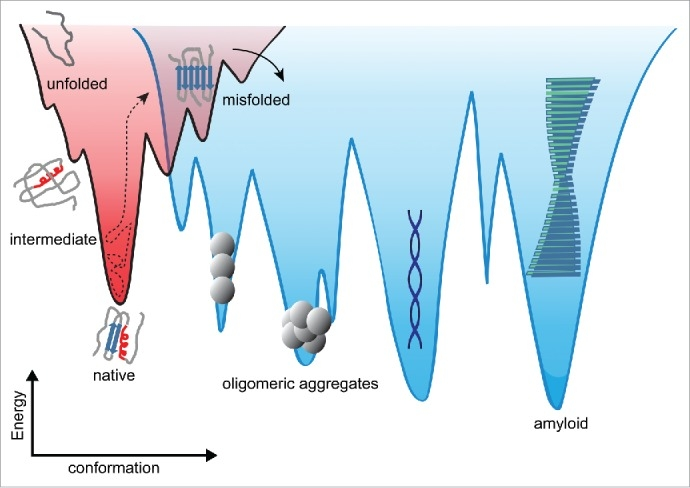
\includegraphics[width=0.9\textwidth]{prions}
\end{figure}

This is also a question for origins of life--Figure \ref {fig:EnergyForOrigin}--\cite{mast2013escalation}
\begin{figure}[H]
	\caption{How do we drive reaction to kinetic state?} \label{fig:EnergyForOrigin} 
	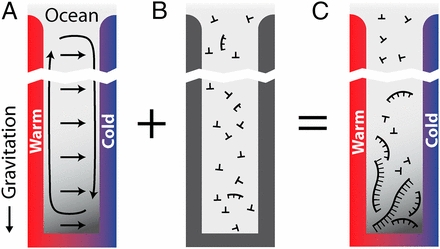
\includegraphics[width=0.9\textwidth]{EnergyForOrigin}
\end{figure}

\textbf{Open Questions}
\begin{itemize}
	\item Do environments exist where biological building
	blocks such as amino acids are
	thermodynamically favored, but exploration of
	their sequence space is kinetically favored?
	\item How do chemical systems utilize environmental
	energy to form kinetic assemblies?
\end{itemize}

See \cite{pross2017and},\cite{semenov2016autocatalytic},\cite{pross2008can}, \cite{pross2005emergence}.

\section{Chemical Configurations: Proteins and DNA}

\section{Early Metabolisms}

\subsection{Introduction}

Lecturer: Kate Adamala


\cite{bar2011survey}, \cite{fuchs2011alternative}, \cite{weiss2016physiology}

\subsection{Energetics}


\section{Energy Harvesting}

\cite{simon2008organisation}

\section{Systematics and Limits of Metabolic Rates}

% end of text 

% glossary
\printglossaries

% bibliography goes here
 
\bibliographystyle{unsrt}
\addcontentsline{toc}{section}{Bibliography}
\bibliography{origins}

\end{document}
